% !Mode:: "TeX:UTF-8:Main"
% arara: pdflatex
% arara: convert: {density: 96, otheroptions: -dispose previous -delay 20 -loop 1, format: gif}
% xarara: showfile: {format: gif}
\documentclass{article}
\usepackage[utf8]{inputenc} %probably not needed ...
\usepackage[T1]{fontenc}
\usepackage{geometry}
\geometry{papersize={128mm,96mm},margin=0.5cm} %\textwidth=11.8, \textheight=8.6
\usepackage[svgnames,x11names]{xcolor}
\usepackage{tikzducks}
\usetikzlibrary{shapes.geometric}
\pagestyle{empty}
\parindent=0pt
\usepackage{animate}
\usepackage{eso-pic}
\usepackage{xfp}
    \pgfmathsetseed{10}

\newcommand{\chrismasduck}{%
    \pgfmathsetmacro\scale{0.3+ 0.1*rnd}
    \pgfmathsetmacro\christmascolor{random(10,75)}
    \pgfmathsetmacro\chrismascolormix{random(0,1)}
    \pgfmathsetmacro\duckhair{random(0,4)}
    \pgfmathsetmacro\duckhaircolor{random(10,100)}
    \ifcase\duckhair
     \tikzset{duckhair/.style={longhair=red!\duckhaircolor!black}}
    \or
     \tikzset{duckhair/.style={shorthair=yellow!\duckhaircolor!brown}}
    \or
     \tikzset{duckhair/.style={crazyhair=teal!\duckhaircolor!white}}
     \else
     \tikzset{duckhair/.style={longhair=Blue3!\duckhaircolor!black}}
    \fi
    \duck[santa=red!80!black,/tikz/duckhair,body={\ifnum \chrismascolormix=0 yellow!\christmascolor!brown\else DarkGoldenrod1!\christmascolor!AntiqueWhite1\fi},jacket=DarkSlateGrey,tie=Crimson,eyebrow]
    }


\tikzset{%
 lines/.style={
    ultra thick,
    line join=round,
    line cap=round
  }, sketch/.style={
    bend right, out=rand*10, in=180-rand*10
  }}

\newcommand\duckscolumns{10}
\newcommand\ducksrows{7}

\begin{document}\pagecolor{SpringGreen4}

\foreach\x in {1,2,...,30}
{
\begin{tikzpicture}[scale=0.5,transform shape,overlay]
\pgfmathsetseed{10}
\foreach \n in {1,...,10}{
  \tikzset{xshift=\fpeval{2*(\n-0.8)/\duckscolumns}\textwidth}%
  \fill [lines, fill=Red1, rounded corners=0.125cm]
    (-1/3,0) to [sketch] (-1/3,2) -- (1/3,2)  to [sketch] (1/3,0);
    }
\pgfmathsetseed{\x}
 \foreach \n in {1,...,10}{
  \tikzset{xshift=\fpeval{2*(\n-0.8)/\duckscolumns}\textwidth}%
  % Wick
  \draw [lines] (0,2) -- ++(0,1/4);
  \tikzset{shift={(0,2+1/8)}, xscale=round(rnd)*2-1,yscale=1+rand/8}
  \foreach \s/\c in {1/yellow,.5/red}
    \path [lines, fill=\c!50!orange, scale=\s]
      (0,0)
      arc (270:180:3/8)
      .. controls ++(0,1/4) and ++(0,-1/4) .. (0,3/2)
      arc (90:0:3/8 and 1) arc (360:270:3/8 and 1/2);
   }
\end{tikzpicture}\newpage}

\end{document}

%
\newcommand\duckscolumns{10}
\newcommand\ducksrows{7}
\pgfmathsetseed{10}
\begin{tikzpicture}
\path (0,0) rectangle (\textwidth,\textheight);
\foreach \x in {1,2,...,\duckscolumns}
 {\foreach \y in {1,2,...,\ducksrows}
 {
  \begin{scope}[overlay,
              xshift=\fpeval{(\x-0.8)/\duckscolumns}\textwidth,
              yshift=\fpeval{(\y-0.8)/\ducksrows}\textheight]
  \begin{scope}[scale=0.35]
  \chrismasduck
  \end{scope}
  \end{scope}
 }}
\end{tikzpicture}
\newpage
\pgfmathsetseed{10}
\begin{tikzpicture}
\path (0,0) rectangle (\textwidth,\textheight);
\foreach \x in {1,2,...,\duckscolumns}
 {\foreach \y in {1,2,...,\ducksrows}
 {
  \begin{scope}[overlay,
              xshift=\fpeval{(\x-0.8)/\duckscolumns}\textwidth,
              yshift=\fpeval{(\y-0.8)/\ducksrows}\textheight]
  \begin{scope}[scale=0.35]
  \chrismasduck
  \end{scope}
  \end{scope}
 }}
\end{tikzpicture}


\end{document}